\documentclass{article}

\usepackage[final]{neurips_2024}

\makeatletter
\renewcommand{\@noticestring}{} % removes conference notice
\makeatother


\usepackage[utf8]{inputenc} % allow utf-8 input
\usepackage[T1]{fontenc}    % use 8-bit T1 fonts
\usepackage{hyperref}       % hyperlinks
\usepackage{url}            % simple URL typesetting
\usepackage{booktabs}       % professional-quality tables
\usepackage{amsfonts}       % blackboard math symbols
\usepackage{nicefrac}       % compact symbols for 1/2, etc.
\usepackage{microtype}      % microtypography
\usepackage{xcolor}         % colors
\usepackage{graphicx}
\usepackage{amsmath}

\title{Predicting probability of scoring a second date }


% The \author macro works with any number of authors. There are two commands
% used to separate the names and addresses of multiple authors: \And and \AND.
%
% Using \And between authors leaves it to LaTeX to determine where to break the
% lines. Using \AND forces a line break at that point. So, if LaTeX puts 3 of 4
% authors names on the first line, and the last on the second line, try using
% \AND instead of \And before the third author name.


\author{%
  Baye-by Come Back\\
  University of California, San Diego\\
  % examples of more authors
  % \And
  % Coauthor \\
  % Affiliation \\
  % Address \\
  % \texttt{email} \\
  % \AND
  % Coauthor \\
  % Affiliation \\
  % Address \\
  % \texttt{email} \\
  % \And
  % Coauthor \\
  % Affiliation \\
  % Address \\
  % \texttt{email} \\
  % \And
  % Coauthor \\
  % Affiliation \\
  % Address \\
  % \texttt{email} \\
}


\begin{document}


\maketitle


% \begin{abstract}
%   The abstract paragraph should be indented \nicefrac{1}{2}~inch (3~picas) on
%   both the left- and right-hand margins. Use 10~point type, with a vertical
%   spacing (leading) of 11~points.  The word \textbf{Abstract} must be centered,
%   bold, and in point size 12. Two line spaces precede the abstract. The abstract
%   must be limited to one paragraph.
% \end{abstract}


\section{Problem Description}

We will be predicting whether participants of a first date will go on a second date from features such as attractiveness, sincerity, intelligence, and ambition. Given the property of our dataset, we will construct a Bayesian Network with hidden variables to model the problem, learn CPTs using Expectation Maximization, and apply exact inference for prediction. We will be analyzing how the raw features affect the hidden variables and how the hidden variables influence the outcome of a second date.

\section{Dataset Source}

We will be using the Kaggle \href{https://www.kaggle.com/datasets/polarbearyap/speed-dating}{\textit{Speed~Dating}} dataset. It contains information from 8,378 participants from the years 2002 to 2004.

Each row represents one participant and their date. We plan to use 3 attributes from the dataset, and for each attribute (attractiveness, intelligence, sincerity), the dataset provides 5 related features.

For example, for \textbf{attractiveness}, the dataset includes:
\begin{itemize}
  \item \texttt{attractive}: Participant's self-rating on attractiveness
  \item \texttt{attractive\_partner}: Participant's rating of their partner's attractiveness
  \item \texttt{attractive\_o}: Partner's rating of the participant's attractiveness during the event
  \item \texttt{attractive\_important}: How important attractiveness is to the participant when choosing a partner
  \item \texttt{pref\_o\_attractive}: How important the participant believes their partner considers attractiveness
\end{itemize}

We will include $5\times 3=15$ features in total for our task.

\section{Methodology}

Given raw features $\vec{X}$, we want to infer the probability of a second date $Y$. We want to build a model using the dataset $V_t = \{\vec{X}_t,Y_t\}$. We constructed 3 hidden variables $\vec{Z} = \{Z_1,Z_2,Z_3\}$, each $Z$ represents an attribute (attractiveness, intelligence, sincerity) and incorporates information from 5 features. We want to find out how the raw features $\vec{X}$ affect the hidden variables $\vec{Z}$ and how the hidden variables $\vec{Z}$ influence the outcome of a second date.


\begin{center}
  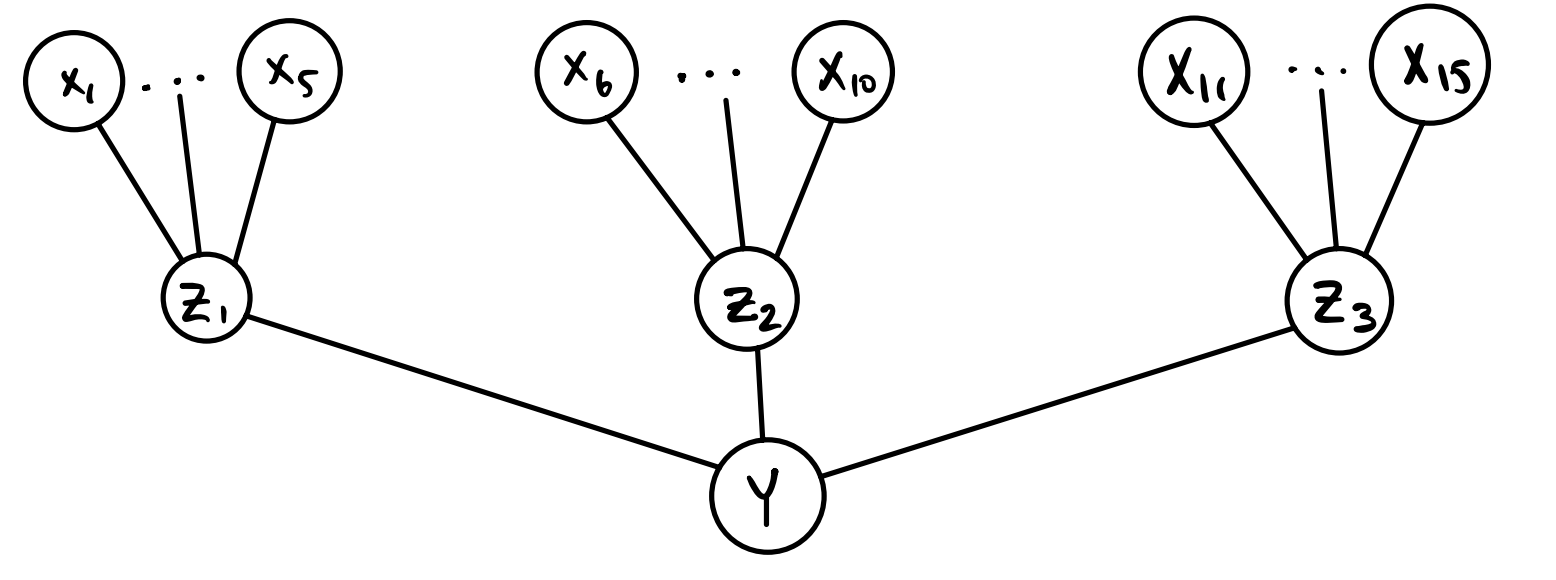
\includegraphics[width=\linewidth]{proposed_model.png}
\end{center}

Let $T$ be the cardinality of the dataset, $x_i$ be the features, $z_i$ be the hidden variables, and $Y \in \{0,1\}$ be whether a second date occurs. We denote $\vec{X^{(i)}} = \{x_{5i-4}, x_{5i-3}, \dots, x_{5i}\}$, $\vec{X} = \{\vec{X}^{(1)},\vec{X}^{(2)},\vec{X}^{(3)}\}$, $\vec{Z} = \{Z_i,Z_2,Z_3\}$.
% We assume x and y to be independent.


\subsection{Learning}

We want to learn the CPTs using Expectation Maximization.


% \[ P(\vec{X},Y) = \sum_Z P(\vec{X})P(Z|\vec{X})P(Y|Z) \]

\subsubsection{E-step}

% \[
% \begin{aligned}
% P(\vec{Z}|\vec{X},Y)
% &= \frac{P(\vec{X},\vec{Z},Y)}{P(\vec{X},Y)}
% = \frac{P(\vec{X})P(\vec{Z}|\vec{X})P(Y|\vec{Z})}{\sum_{\vec{Z'}}P(\vec{X},\vec{Z'},Y)}
% = \frac{P(\vec{X})P(\vec{Z}|\vec{X})P(Y|\vec{Z})}{\sum_{\vec{Z'}}P(\vec{X})P(\vec{Z'}|\vec{X})P(Y|\vec{Z'})} \\
% &= \frac{P(\vec{Z}|\vec{X})P(Y|\vec{Z})}{\sum_{\vec{Z'}}P(\vec{Z'}|\vec{X})P(Y|\vec{Z'})}
% \end{aligned}
% \]

$$
  \begin{aligned}
    P(\vec{Z} | \vec{X}, Y)
     & =  \frac{P(\vec{Z}, Y | \vec{X})}{P(Y | \vec{X})}
    = \frac{P(\vec{Z} | \vec{X})P(Y | \vec{Z})}{\sum_{\vec{Z'}} P(\vec{Z'}, Y | \vec{X})}                                      \\
     & = \frac{P(Y|\vec{Z})\prod_{i=1}^3P(Z_i|\vec{X}^{(i)})}{\sum_{\vec{Z'}} P(Y|\vec{Z'})\prod_{i=1}^3P(Z'_i|\vec{X}^{(i)})}
  \end{aligned}
$$

$$
  \begin{aligned}
    P(Z_i | \vec{X}, Y) = \sum_{Z_j, j\neq i} P(\vec{Z} | \vec{X}, Y)
  \end{aligned}
$$

\subsubsection{M-step}

% Root nodes:

% \[ P(\vec{X}) \leftarrow \frac{\sum_{i=1}^T P(\vec{X}|\vec{X}_i,Y_i)}{T} = \frac{\sum_{i=1}^T I(\vec{X},\vec{X}_i)}{T} \]

% Nodes with parents:

$$
  \begin{aligned}
    P(Z_i|\vec{X^{(i)}})
     & \leftarrow \frac{\sum_{t=1}^T P(Z_i,\vec{X^{(i)}} | \vec{X}_t, Y_t)}{\sum_{t=1}^T P(\vec{X^{(i)}}| \vec{X}_t, Y_t)}
    = \frac{\sum_{t=1}^T I(\vec{X^{(i)}},  \vec{X^{(i)}_t}) P(Z_i | \vec{X}_t, Y_t)}{\sum_{t=1}^T I(\vec{X^{(i)}},  \vec{X^{(i)}_t})} \\
  \end{aligned}
$$

$$
  \begin{aligned}
    P(Y|\vec{Z})
     & \leftarrow \frac{\sum_{t=1}^T P(Y,\vec{Z} | \vec{X}_t, Y_t)}{\sum_{t=1}^T P(\vec{Z}| \vec{X}_t, Y_t)}
    = \frac{\sum_{t=1}^T I(Y,  Y_t) P(\vec{Z} | \vec{X}_t, Y_t)}{\sum_{t=1}^T P(\vec{Z}| \vec{X}_t, Y_t)}    \\
  \end{aligned}
$$

% \[ P(\vec{Z}|\vec{X}) \leftarrow \frac{\sum_{i=1}^T P(\vec{X},Z|\vec{X}_i,Y_i)}{\sum_{i=1}^TP(\vec{X}|\vec{X}_i,Y_i)} = \frac{\sum_{i=1}^T I(\vec{X},\vec{X}_i) P(\vec{Z}|\vec{X}_i,Y_i)}{\sum_{i=1}^T I(\vec{X},\vec{X}_i)} \]

% \[ P(Y|\vec{Z}) \leftarrow \frac{\sum_{i=1}^T P(Y,\vec{Z}|\vec{X}_i,Y_i)}{\sum_{i=1}^T P(Z|\vec{X}_i,Y_i)} = \frac{\sum_{i=1}^T I(Y,Y_i) P(\vec{Z}|\vec{X}_i,Y_i)}{\sum_{i=1}^T P(Z|\vec{X}_i,Y_i)} \]

\subsection{Inference}


\[
  \begin{aligned}
    P(Y=1 | \vec{X})
     & = \sum_{\vec{Z}} P(Y=1, \vec{Z} | \vec{X}) = \sum_{\vec{Z}} P(\vec{Z} |\vec{X}) P(Y = 1|\vec{Z}) \\
     & = \sum_{\vec{Z}}P(Y=1|\vec{Z})\prod_{i=1}^3P(Z_i|\vec{X}^{(i)})
  \end{aligned}
\]


\end{document}